\documentclass[a4paper, 12pt]{report}
\usepackage[utf8]{inputenc}
\usepackage{tikz}
\usepackage{graphicx}
\usepackage{geometry}
\geometry{margin=1in,left=0.6in,right=0.6in,bottom=0.5in}
\usepackage{fancyhdr}
\usepackage{hyperref}
\usepackage{chemfig}
\usetikzlibrary{calc}
\usepackage{enumitem}
\usepackage{placeins}
\usepackage{caption}
\usepackage{array}
\usepackage{float}
\usepackage{amsmath, amssymb, amscd, MnSymbol,mathrsfs}
\usepackage{tcolorbox}
\usepackage{bibref}
\usepackage{bm}
\newcommand{\vect}[1]{\boldsymbol{\mathbf{#1}}}

\usepackage{empheq}
\usepackage{pgfplots}
\pgfplotsset{compat=1.18}
\usetikzlibrary{calc, angles, quotes}
\usepackage{circuitikz}
\usepackage{booktabs}
\usepackage{array}
\usepackage{arydshln}
\usepackage{tcolorbox}

\usepackage{hyperref}
\usepackage{cancel}
\usepackage{changepage}
\usepackage{placeins}
\usepackage{enumitem}
\usepackage{pgf}


\usepackage{listings}
\usepackage{courier}
\usepackage{xcolor}
\usepackage{color}

\lstdefinestyle{mypythonstyle}{
    language=Python,
    basicstyle=\footnotesize\ttfamily,
    numbers=left,
    numberstyle=\tiny,
    numbersep=5pt,
    showstringspaces=false,
    frame=single,
    breaklines=true,
    keywordstyle=\color{blue},
    commentstyle=\color{green!60!black},
    stringstyle=\color{red},
    backgroundcolor=\color{gray!10},
}


\makeatletter
\renewcommand*\env@matrix[1][\arraystretch]{%
    \edef\arraystretch{#1}%
    \hskip -\arraycolsep
    \let\@ifnextchar\new@ifnextchar
    \array{*{\c@MaxMatrixCols}c}
}
\makeatother


\pagestyle{fancy}
\fancyhf{}
\fancyhead[L]{Module: EG4017 - Engineering Mathematics}
\fancyhead[R]{Page \thepage}

\title{\vspace{3em} \Huge \textbf{Engineering\\ Mathematics and Computing}\\ \vspace{1em} \Large Task 1: Coursework Assessment}
\author{Student Name: Sakariye Abiikar\\ KID: 2371673}
\date{Last Updated: October 19, 2024\\ Submission Deadline: November 7, 2024, 5pm \\[1em] Git Repo : \color{blue}\url{https://github.com/sakx7/mathcompuni}}

\begin{document}
    
    \maketitle
    \thispagestyle{empty}
    
    \newpage
    \thispagestyle{empty}
    \newgeometry{margin=1in,left=0.6in,right=0.6in,bottom=0in}

    \chapter{Part A: Mathematics}
    \hrule\vspace{5em}\Large\noindent
    \textbf{Notes:}\normalsize
    
    %\begin{itemize}
    %    \item \textbf{Module Code:} EG4017
    %    \item \textbf{Module Title:} Engineering Mathematics
    %    \item \textbf{Assessment Title:} Engineering Mathematics and Computing - Task 1
    %    \item \textbf{Summative Assessment:} This assignment contributes 50\% of module grade.
    %    \item \textbf{Total Hours Required:} 25 hours per student
    %    \item \textbf{Set by:} Dr. Sergey Khaustov (RVMB122)
    %    \item \textbf{Contact:} S.Khaustov@kingston.ac.uk
    %    \item \textbf{Submission Deadline:} November 7, 2024, before 5pm
    %    \item \textbf{Feedback Release:} Formal feedback will be provided %within 20 working days after submission.
    %\end{itemize}
    
    
    \newpage\centering\restoregeometry
    
    \setcounter{page}{1}
    \fancyhead[L]{Part A: Mathematics}

    \begin{tcolorbox}[title={\color{black}{\section{Q1}}}, colback=white, colframe=black!30!white, boxrule=0.4mm, width=1\textwidth]
        Use the quotient rule to differentiate the function \( y=\frac{\ln 3 x}{2 x} \)
    \end{tcolorbox}
    
    The quotient rule states that if
    \[y = \frac{u}{v} \quad \text{then} \quad y' = \frac{u'v - uv'}{v^2}\]
    Here: \\[5pt]
    \begin{minipage}{0.4\textwidth}
        \[u = \ln 3x\] 
    \end{minipage}\hspace{-8em}
    \begin{minipage}{0.4\textwidth}
        \[v = 2x \]
    \end{minipage}\\[20pt]
    First, find the derivatives:\\[10pt]
    \begin{minipage}{0.43\textwidth}\centering
    \[u = \ln(3x)\]
    Let:
    \[\delta = 3x \qquad u = \ln(\delta)\]
    \[\frac{du}{d\delta} = \frac{1}{\delta} \qquad \frac{d\delta}{dx} = 3\]
    Using the chain rule, we can find:
    \[\frac{du}{dx} = \frac{du}{d\delta} \cdot \frac{d\delta}{dx}\]
    \[\frac{du}{dx} = \frac{3}{\delta} = \frac{3}{3x}= \frac{1}{x}\]
    General rule for composite/nested functions is solved via chain rule it's:
    \[\frac{d}{dx}(f(g(x))) = f'(g(x))\cdot g'(x)\]
    \end{minipage}\hspace{1em}\vrule\hspace{-2.5em}
    \begin{minipage}{0.4\textwidth}
        \[v = 2x\]
        \[v' = \frac{d}{dx}(2x) = 2\]
    \end{minipage}\\[30pt]
    Now we can apply the quotient rule:
    \[y' = \frac{\left(\frac{1}{x}\right)(2x) - (\ln 3x)(2)}{(2x)^2} = \frac{2 - 2\ln 3x}{4x^2}\]
    \[\boxed{y' = \frac{1 - \ln 3x}{2x^2}}\]
    
    \newpage
    \begin{tcolorbox}[title=\color{black}{\section{Q2}}, colback=white, colframe=black!30!white, boxrule=0.4mm, width=1\textwidth]
        Find the angle between the vectors \( 2 i-11 j-10 k \) and \( 5 i+8 j+7 k \)
    \end{tcolorbox}
    
    The angle \( \theta \) between two vectors \(\mathbf{a}\) and \(\mathbf{b}\) is given by:
    \[\cos \theta = \frac{\mathbf{a} \cdot \mathbf{b}}{\|\mathbf{a}\| \|\mathbf{b}\|}\]
    Calculate the dot product:
    \[\mathbf{a} \cdot \mathbf{b} = \underbrace{(2)(5)}_i + \underbrace{(-11)(8)}_j + \underbrace{(-10)(7)}_k = -148\]
    Calculate the magnitudes:
    \[\|\mathbf{a}\| = \sqrt{2^2 + (-11)^2 + (-10)^2} = \sqrt{225} = 15\]
    \[\|\mathbf{b}\| = \sqrt{5^2 + 8^2 + 7^2} = \sqrt{138}\]
    Find \(\cos \theta\):
    \[\cos \theta = \frac{-148}{15 \times \sqrt{138}}\]
    Thus, the angle \(\theta\) is:
    \[\boxed{\theta = \cos^{-1}\left(\frac{-148}{15 \times \sqrt{138}}\right) \approx 147.1^{\circ}}\]
    
    \newpage    
    \begin{tcolorbox}[title=\color{black}{\section{Q3}}, colback=white, colframe=black!30!white, boxrule=0.4mm, width=1\textwidth]
        Find the rate of change of \( y=\ln \left(16 t^{2}+19\right) \) at the specified point \( t=9 \)
    \end{tcolorbox}
        
    Differentiate \( y \) with respect to \( t \):\\[1em]
    Note prior (q1) that the general rule for composite/nested functions is:
    \[\frac{d}{dx}(f(g(x))) = f'(g(x))\cdot g'(x)\]
    Here for $y=\ln \left(16 t^{2}+19\right)$
    \[\frac{dy}{dt} = \frac{1}{16t^2 + 19} \cdot \frac{d}{dt}(16t^2 + 19)\]
    \[\frac{d}{dt}(16t^2 + 19) = 32t\]
    \[\frac{dy}{dt} = \frac{1}{16t^2 + 19} \cdot 32t = \frac{32t}{16t^2 + 19}\]
    Evaluate at \( t = 9 \):
    \[\boxed{\frac{dy}{dt} \bigg|_{t=9} = \frac{32 (9)}{16(9)^2 + 19} = \frac{288}{1315} \approx 0.219}\]
    
    \newpage
    \begin{tcolorbox}[title=\color{black}{\section{Q4}}, colback=white, colframe=black!30!white, boxrule=0.4mm, width=1\textwidth]
        Express \( \cos t-8 \sin t \) in the form \( A \cos (\omega t+\alpha) \), where \( \alpha \geq 0 \)
    \end{tcolorbox}
    you see the thing is the left side, \( \cos t - 8 \sin t \), is standard, but the right side introduces a different frequency, \( \omega \), in \( A \cos (\omega t + \alpha) \).\\[10pt]
    Since the left side has a frequency of 1, im just gonna assume \( \omega = 1 \) for simplicity. If \( \omega \) were different, you would need to rewrite the left side in terms of \( \omega t \), but this isn't specified in the problem.\\
    \vspace{0.5em}\hrule\vspace{0.5em}
    The angle subtraction formula is:
    \[A \cos(t - \phi) = A \cos(\phi) \cos(t) + A \sin(\phi) \sin(t)\]
    By comparing coefficients from both sides, we have:
    \begin{align*}
        a & = A \cos(\phi) \\
        b & = A \sin(\phi)
    \end{align*}
    To find $A$ we use $A = \sqrt{a^2 + b^2}$\\
    \vspace*{1em}
    \begin{minipage}{0.45\textwidth}\centering
        This arises from squaring both equations \(a = A \cos(\phi)\) and \(b = A \sin(\phi)\):\\[1em]
        $a^2 + b^2 = (A \cos(\phi))^2 + (A \sin(\phi))^2 = A^2 (\cos^2(\phi) + \sin^2(\phi)) = A^2$
    \end{minipage}\\
    
    \vspace{1em}
    To find the phase shift \(\phi\), we use $\tan \phi = \frac{b}{a}$\\[1em]
    \begin{minipage}{0.45\textwidth}\centering
        This comes from the definitions of sine and cosine:
        \[\tan \phi = \frac{A \sin(\phi)}{A \cos(\phi)} = \frac{b}{a}\]
    \end{minipage}\\
    \vspace{1em}
    In so we derive and make use of:
    \[A \cos(t - \phi) = a \cos(t) + b \sin(t)\]
    Where $A = \sqrt{a^2 + b^2}$ and $\tan \phi = \frac{b}{a}$\\
    \vspace{0.5em}\hrule\vspace{0.5em}
    for $b=-8$ and $a=2$
    \[A = \sqrt{1^2 + (-8)^2} = \sqrt{65}\]
    \[\tan \phi = \frac{-8}{1}=-8 \qquad \phi = \arctan(-8) \approx -82.87^\circ\]\\[6pt]
    In so plugging in gives
    \begin{align*}
    \cos t-8 \sin t &= A \cos(t - \phi)\\
    &= \sqrt{65} \cos(t - \arctan(-8))\\
    &= \sqrt{65} \cos(t - (-82.87^\circ))   
    \end{align*}
    \[\boxed{\cos t-8 \sin t \approx  8.06 \cos(t + 82.87^\circ)}\]
    
    \newpage
    \begin{tcolorbox}[title=\color{black}{\section{Q5}}, colback=white, colframe=black!30!white, boxrule=0.4mm, width=1\textwidth]
        Solve the following system of three linear equations using Cramer's rule
        \[
        \left\{\begin{array}{c}
            11 v_{1}-v_{2}+v_{3}=31.4 \\
            v_{1}+\frac{v_{2}}{2}-v_{3}=1.9 \\
            -9 v_{1}+11 v_{3}=-12
        \end{array}\right.
        \]
    \end{tcolorbox}
    
    The system can be written in matrix form \( A\mathbf{v} = \mathbf{b} \), specifically because of the variable distributions where:
    \[A = \begin{bmatrix} 11 & -1 & 1 \\ 1 & \frac{1}{2} & -1 \\ -9 & 0 & 11 \end{bmatrix}, \quad \mathbf{v} = \begin{bmatrix} v_1 \\ v_2 \\ v_3 \end{bmatrix}, \quad \mathbf{b} = \begin{bmatrix} 31.4 \\ 1.9 \\ -12 \end{bmatrix}\]
    Calculate the determinant \(\det(A)\).
    \[\det(A) = 67\]
    Now solve for each variable using Cramer's rule:
    \[A_1 = \begin{bmatrix} 31.4 & -1 & 1 \\ 1.9 & \frac{1}{2} & -1 \\ -12 & 0 & 11 \end{bmatrix}
    \quad 
    A_2 = \begin{bmatrix} 11 & 31.4 & 1 \\ 1 & 1.9 & -1 \\ -9 & -12 & 11 \end{bmatrix}
    \quad 
    A_3 = \begin{bmatrix} 11 & -1 & 31.4 \\ 1 & \frac{1}{2} & 1.9 \\ -9 & 0 & -12 \end{bmatrix}\]
    Calculate the determinants:
    \[\det(A_1)\approx187.6 \quad \det(A_2)\approx40.2\quad \det(A_3)\approx80.4\]
    \(\mathbf{v}\) can be found as:
    \[v_1 = \frac{\det(A_1)}{\det(A)}, \quad v_2 = \frac{\det(A_2)}{\det(A)}, \quad v_3 = \frac{\det(A_3)}{\det(A)}\]
    \[\boxed{\begin{array}{rcl}v_1=\frac{187.6}{67}=2.8\\[6pt]v_2=\frac{40.2}{67}=0.6\\[6pt]v_3=\frac{80.4}{67}=1.2\end{array}}\]
    There are a few ways to calculate the determinants, but especially in this working out i chose not show the method i used since it’s not the main focus of the question.\\[6pt]
    If you’re curious about how I did it, the Sarrus method for simplicity.
    \newpage    
    \begin{tcolorbox}[title=\color{black}{\section{Q6}}, colback=white, colframe=black!30!white, boxrule=0.4mm, width=1\textwidth]
        Transpose \( z = d + a \sqrt{y} \) to make \( y \) the subject.
    \end{tcolorbox}

    Starting with:
    \[z = d + a\sqrt{y}\]
    \[z - d = a\sqrt{y}\]
    \[\frac{z - d}{a} = \sqrt{y}\]
    \[\left( \frac{z - d}{a} \right)^2 = y\]
    Thus, the expression for \( y \) is:
    \[\boxed{y = \frac{(z - d)^2}{a^2}}\]
    i generally consider this the most concise and general expression for $y$.\\
    im aware you could expand \( (z - d)^2 \):
    \[y = \frac{z^2 - 2zd + d^2}{a^2}\]
    and additionally take into account of both possible factorisations:
    \[y = \frac{z^2+d(d-2z)}{a^2}\]
    \[y = \frac{d^2+z(z-2d)}{a^2}\]    
    
    \newpage
    \begin{tcolorbox}[title=\color{black}{\section{Q7}}, colback=white, colframe=black!30!white, boxrule=0.4mm, width=1\textwidth]
        Find a vector that is perpendicular to both of the vectors $$ \boldsymbol{a}=4 \boldsymbol{i}+3 \boldsymbol{j}+5 \boldsymbol{k} $$$$ \boldsymbol{b}=3 \boldsymbol{i}+4 \boldsymbol{j}-6 \boldsymbol{k} $$ Hence find a unit vector that is perpendicular to both \( \boldsymbol{a} \) and \( \boldsymbol{b} \).
    \end{tcolorbox}
    
    The unit vector is
    \[\mathbf{\hat{r}} =\frac{\vec{r}}{||{\vec{r}}||}\]
    Here we want to define $\vec{r}$ as a vector perpendicular to both $\mathbf{a}$ and $\mathbf{b}$, to do that we take there cross product \(\mathbf{a} \times \mathbf{b}\)
    \[\vec{r}=\mathbf{a} \times \mathbf{b} = \begin{vmatrix} \mathbf{i} & \mathbf{j} & \mathbf{k} \\ 4 & 3 & 5 \\ 3 & 4 & -6 \end{vmatrix}= -38\mathbf{i} + 39\mathbf{j} + 7\mathbf{k}\]
    Find the magnitude:
    \[||{\vec{r}}||=\|\mathbf{a} \times \mathbf{b}\| = \sqrt{(-38)^2 + 39^2 + 7^2} = \sqrt{3014}\]
    The unit vector is:
    \[\boxed{\frac{-38\mathbf{i} + 39\mathbf{j} + 7\mathbf{k}}{\sqrt{3014}}}\]

    \newpage
    \begin{tcolorbox}[title=\color{black}{\section{Q8}}, colback=white, colframe=black!30!white, boxrule=0.4mm, width=1\textwidth]
        If \( M=\left(\begin{array}{cc}7 & 9 \\ 1 & -2\end{array}\right) \) and \( N=\left(\begin{array}{cc}2 & 1 \\ -2 & 6\end{array}\right) \) find \( M N \) and \( N M \)
    \end{tcolorbox}
    
    Calculate \( MN \):
    \[MN = \begin{bmatrix} 7 & 9 \\ 1 & -2 \end{bmatrix} \begin{bmatrix} 2 & 1 \\ -2 & 6 \end{bmatrix}\]
    \[= \begin{bmatrix} 7 \cdot 2 + 9 \cdot (-2) & 7 \cdot 1 + 9 \cdot 6 \\ 1 \cdot 2 + (-2) \cdot (-2) & 1 \cdot 1 + (-2) \cdot 6 \end{bmatrix}\]
    \[\boxed{= \begin{bmatrix} -4 & 61 \\ 6 & -11 \end{bmatrix}}\]
    Calculate \( NM \):
    \[NM = \begin{bmatrix} 2 & 1 \\ -2 & 6 \end{bmatrix} \begin{bmatrix} 7 & 9 \\ 1 & -2 \end{bmatrix}\]
    \[= \begin{bmatrix} 2 \cdot 7 + 1 \cdot 1 & 2 \cdot 9 + 1 \cdot (-2) \\ -2 \cdot 7 + 6 \cdot 1 & -2 \cdot 9 + 6 \cdot (-2) \end{bmatrix}\]
    \[\boxed{= \begin{bmatrix} 15 & 16 \\ -8 & -30 \end{bmatrix}}\]
    
    \newpage
    \begin{tcolorbox}[title=\color{black}{\section{Q9}}, colback=white, colframe=black!30!white, boxrule=0.4mm, width=1\textwidth]
        If \( y=x^{4}-4 x^{3}-90 x^{2} \), find the values of \( x \) for which \( y^{\prime \prime}=0 \)
    \end{tcolorbox}
    
    First, find the first derivative:
    \[y' = \frac{d}{dx}(x^4 - 4x^3 - 90x^2) = 4x^3 - 12x^2 - 180x\]
    Find the second derivative:
    \[y'' = \frac{d}{dx}(4x^3 - 12x^2 - 180x) = 12x^2 - 24x - 180\]
    Set \( y'' = 0 \):
    \[12x^2 - 24x - 180 = 0\]
    Divide by 12:
    \[x^2 - 2x - 15 = 0\]
    Factor:
    \[(x - 5)(x + 3) = 0\]
    \[\boxed{x = 5,\ x = -3}\]
    
    \newpage
    \begin{tcolorbox}[title=\color{black}{\section{Q10}}, colback=white, colframe=black!30!white, boxrule=0.4mm, width=1\textwidth]
        Transpose \( b=g+t(a-3) \) to make \( a \) the subject
    \end{tcolorbox}
    
    Starting with:
    \[b = g + t(a - 3)\]
    this is easily rearranged to isolate \( a \):
    \[b - g = t(a - 3)\]
    \[\frac{b - g}{t} = a - 3\]
    \[\boxed{a = \frac{b - g}{t} + 3}\]
    
    \newpage\raggedright
    \thispagestyle{empty}
    \newgeometry{margin=1in,left=0.6in,right=0.6in,bottom=0in}
    
    \chapter{Part B: Computing}

    \hrule
    \vspace{3em}
    \begin{center}
        \Large\textbf{Notes:}
    \end{center}
    \vspace{1em}
    \begin{itemize}
        \item All graphs and images have been coded in TikZ PGF by yours truly.
        \item Code implementations are also original work.
        \item Please evaluate the answer to the questions in its whole. 
    \end{itemize}
    
    \vspace{1em}
    
    \section*{Interpretation of Module Learning Outcomes}
    
    The module learning outcomes are seen as flexible guidelines that promote mastery of mathematical concepts alongside creative problem-solving approaches. This interpretation is supported by the following perspectives:
    
    \begin{enumerate}
        \item \textbf{Diverse Language Utilization:} While \textbf{MATLAB} is specifically mentioned, the focus seems to be on demonstrating mathematical proficiency rather than adhering to a particular programming language. This opens the essentially lets me use tools like Python or R to effectively illustrate an understanding of the concepts. I will strive to align my work with MATLAB where possible.\\[1em]
        But because of MATLAB's drawbacks—for instance, it's not free—I frequently find myself adopting alternatives. These come with difficulties including restricted access and a lack of software expertise. In general, I find it to be rather annoying.  
                
        \item \textbf{Understanding Over Language Proficiency:} The assessment values comprehension of mathematical methods and their application more than expertise in a specific software environment. This perspective enables the presentation of clear, well-documented solutions that reflect a solid understanding of the material, regardless of the medium employed.
    \end{enumerate}

    \newpage
    \setcounter{page}{11}
    \centering
    \fancyhead[L]{Part B: Computing}
    \newpage
    \newgeometry{margin=1in,left=0.6in,right=0.6in,bottom=0.5in}
   \begin{tcolorbox}[title=\color{black}{\section{Q1}}, colback=white, colframe=black!30!white, boxrule=0.4mm, width=1\textwidth]\centering
    The arc length of a segment of a parabola \(ABC\) of an ellipse with semi-minor axes \(a\) and \(b\) is given
    approximately by:
    \[L_{ABC} = \frac{1}{2}\sqrt{b^2+16a^2}+\frac{b^2}{8a}\ln\left(\frac{4a+\sqrt{b^2+16a^2}}{b}\right)\]
    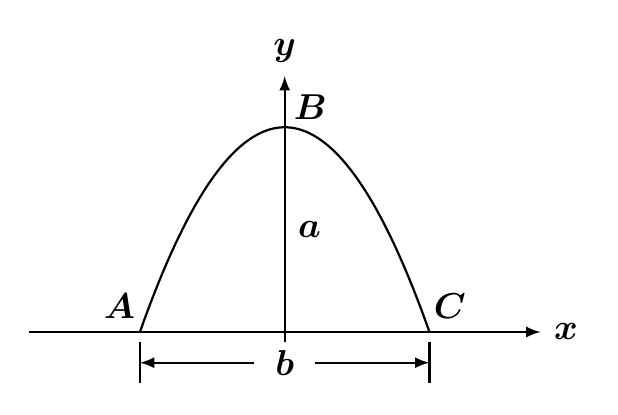
\begin{tikzpicture}[scale=1.3,transform shape,thick]
        \def\a{2} %main parameter
        \pgfmathsetmacro{\asqrt}{sqrt(\a)}
        \begin{scope}
            \clip (\asqrt+0.1, 0) rectangle (-\asqrt-0.1, \a+0.1);
            \draw[domain=-\asqrt:\asqrt, samples=100, smooth] plot (\x, {-(\x)^2 + \a});
        \end{scope}
        \draw[-latex] (-2.5, 0) -- (2.5, 0) node[right] {$\bm{x}$};
        \draw[-latex] (0, -0.1) -- (0, \a+0.5) node[above] {$\bm{y}$};%set reletive to 'a'can be changed
        \node[right] at (0, \a/2) {$\bm{a}$};
        \node at (-\asqrt-0.2, 0.25) {$\bm{A}$};
        \node at (\asqrt+0.2, 0.25) {$\bm{C}$};
        \node at (0.25,\a+0.2 ) {$\bm{B}$};
  
        \def\pad{0.3}
        \def\lin{0.2}
        \begin{scope}[shift={(0,-0.1)}]
             \draw[latex-] (-\asqrt, -0.2) -- (-\pad, -0.2);
            \draw[-latex] (\pad, -0.2) -- (\asqrt, -0.2);
            \node at (0,-0.2) {$\bm{b}$};
            \draw[-] (-\asqrt, -0.2+\lin) -- (-\asqrt, -0.2-\lin);
            \draw[-] (\asqrt, -0.2+\lin) -- (\asqrt, -0.2-\lin);
        \end{scope}
    \end{tikzpicture}\\[1em]
    Write a universal, user-friendly code, test your programme and determine $L_{ABC}$ if $a=11$ cm and $b=9$ cm.
    \end{tcolorbox}
    

    We are tasked with analyzing a parabola where:\\
    \vspace{1em}
    \hspace{3.8em}
    \begin{minipage}{0.6\textwidth}\centering
    \begin{itemize}[itemsep=-0.1cm]
        \item $a$ represents the height of the parabola
        \item $b$ represents the width of the parabola
    \end{itemize}
    \end{minipage}\\
    \vspace*{1em}
    
    To plot the parabola, we must first formulate an equation in terms of these factors. Initially, we begin with a simple parabola in the general shape shown in the graph. Our goal is to select a reasonable function, with variables associated with the $x$ scale and $y$ location of the parabola:    
    \[y = -(\beta x)^2 + \gamma\]
    Given our problem statement:\\
    \vspace{1em}
    \hspace{3.8em}
    \begin{minipage}{0.8\textwidth}\centering
       \begin{itemize}[itemsep=-0.1cm]
        \item $\gamma$ represents the height, so $\gamma = a$
        \item The width is related to the roots of the equation when $y = 0$
    \end{itemize}
    \end{minipage}\\
    \vspace{1em}
    To find $\beta$, we solve:
    \[0 = -(\beta x)^2 + \gamma\]
    \[\beta = \frac{2\sqrt{\gamma}}{b}\]
    since we know $\gamma$:
    \[\beta = \frac{2\sqrt{a}}{b}\]
    Note: This requires $b \neq 0$ and $\sqrt{a} \neq 0$ (i.e., $a > 0$).\\
    Substituting $\gamma$ and $\beta$ into our original equation:
    \[\boxed{y = -\left(\frac{2\sqrt{a}}{b}x\right)^2 + a}\]
    This is our final parabola equation in terms of $a$ and $b$.
    \newpage
    
    The arc length of the parabola from $x = -\frac{b}{2}$ to $x = \frac{b}{2}$ is given by:
    \[L_{ABC} = \frac{1}{2}\sqrt{b^2 + 16a^2} + \frac{b^2}{8a}\ln\left(\frac{4a + \sqrt{b^2 + 16a^2}}{b}\right)\]
    When implementing this in a program:
    \begin{itemize}[itemsep=-0.1cm]
        \item Ensure that when there are no limit parameters for the inputs \(a\) and \(b\), the conditions \(a > 0\) and \(b \neq 0\) are appropriately handled.
        \item Update the plot of \(y = -\left(\frac{2\sqrt{a}}{b}x\right)^2 + a\) so that the sliders for \(a\) and \(b\) directly control the height and width, respectively.
        \item Calculate the arc length of the parabola using a function with inputs \(a\) and \(b\), and display the result in the plot.
    \end{itemize}
    \raggedright
    
    The rest is just nitpicky presentation, all just preference.
    
    \centering
    \lstinputlisting[style=mypythonstyle, title=\textbf{\textcolor{blue}{\texttt{\href{https://github.com/sakx7/mathcompuni/blob/main/scripts/q1.py}{scripts/q1.py}}}}]{scripts/q1.py}
    
    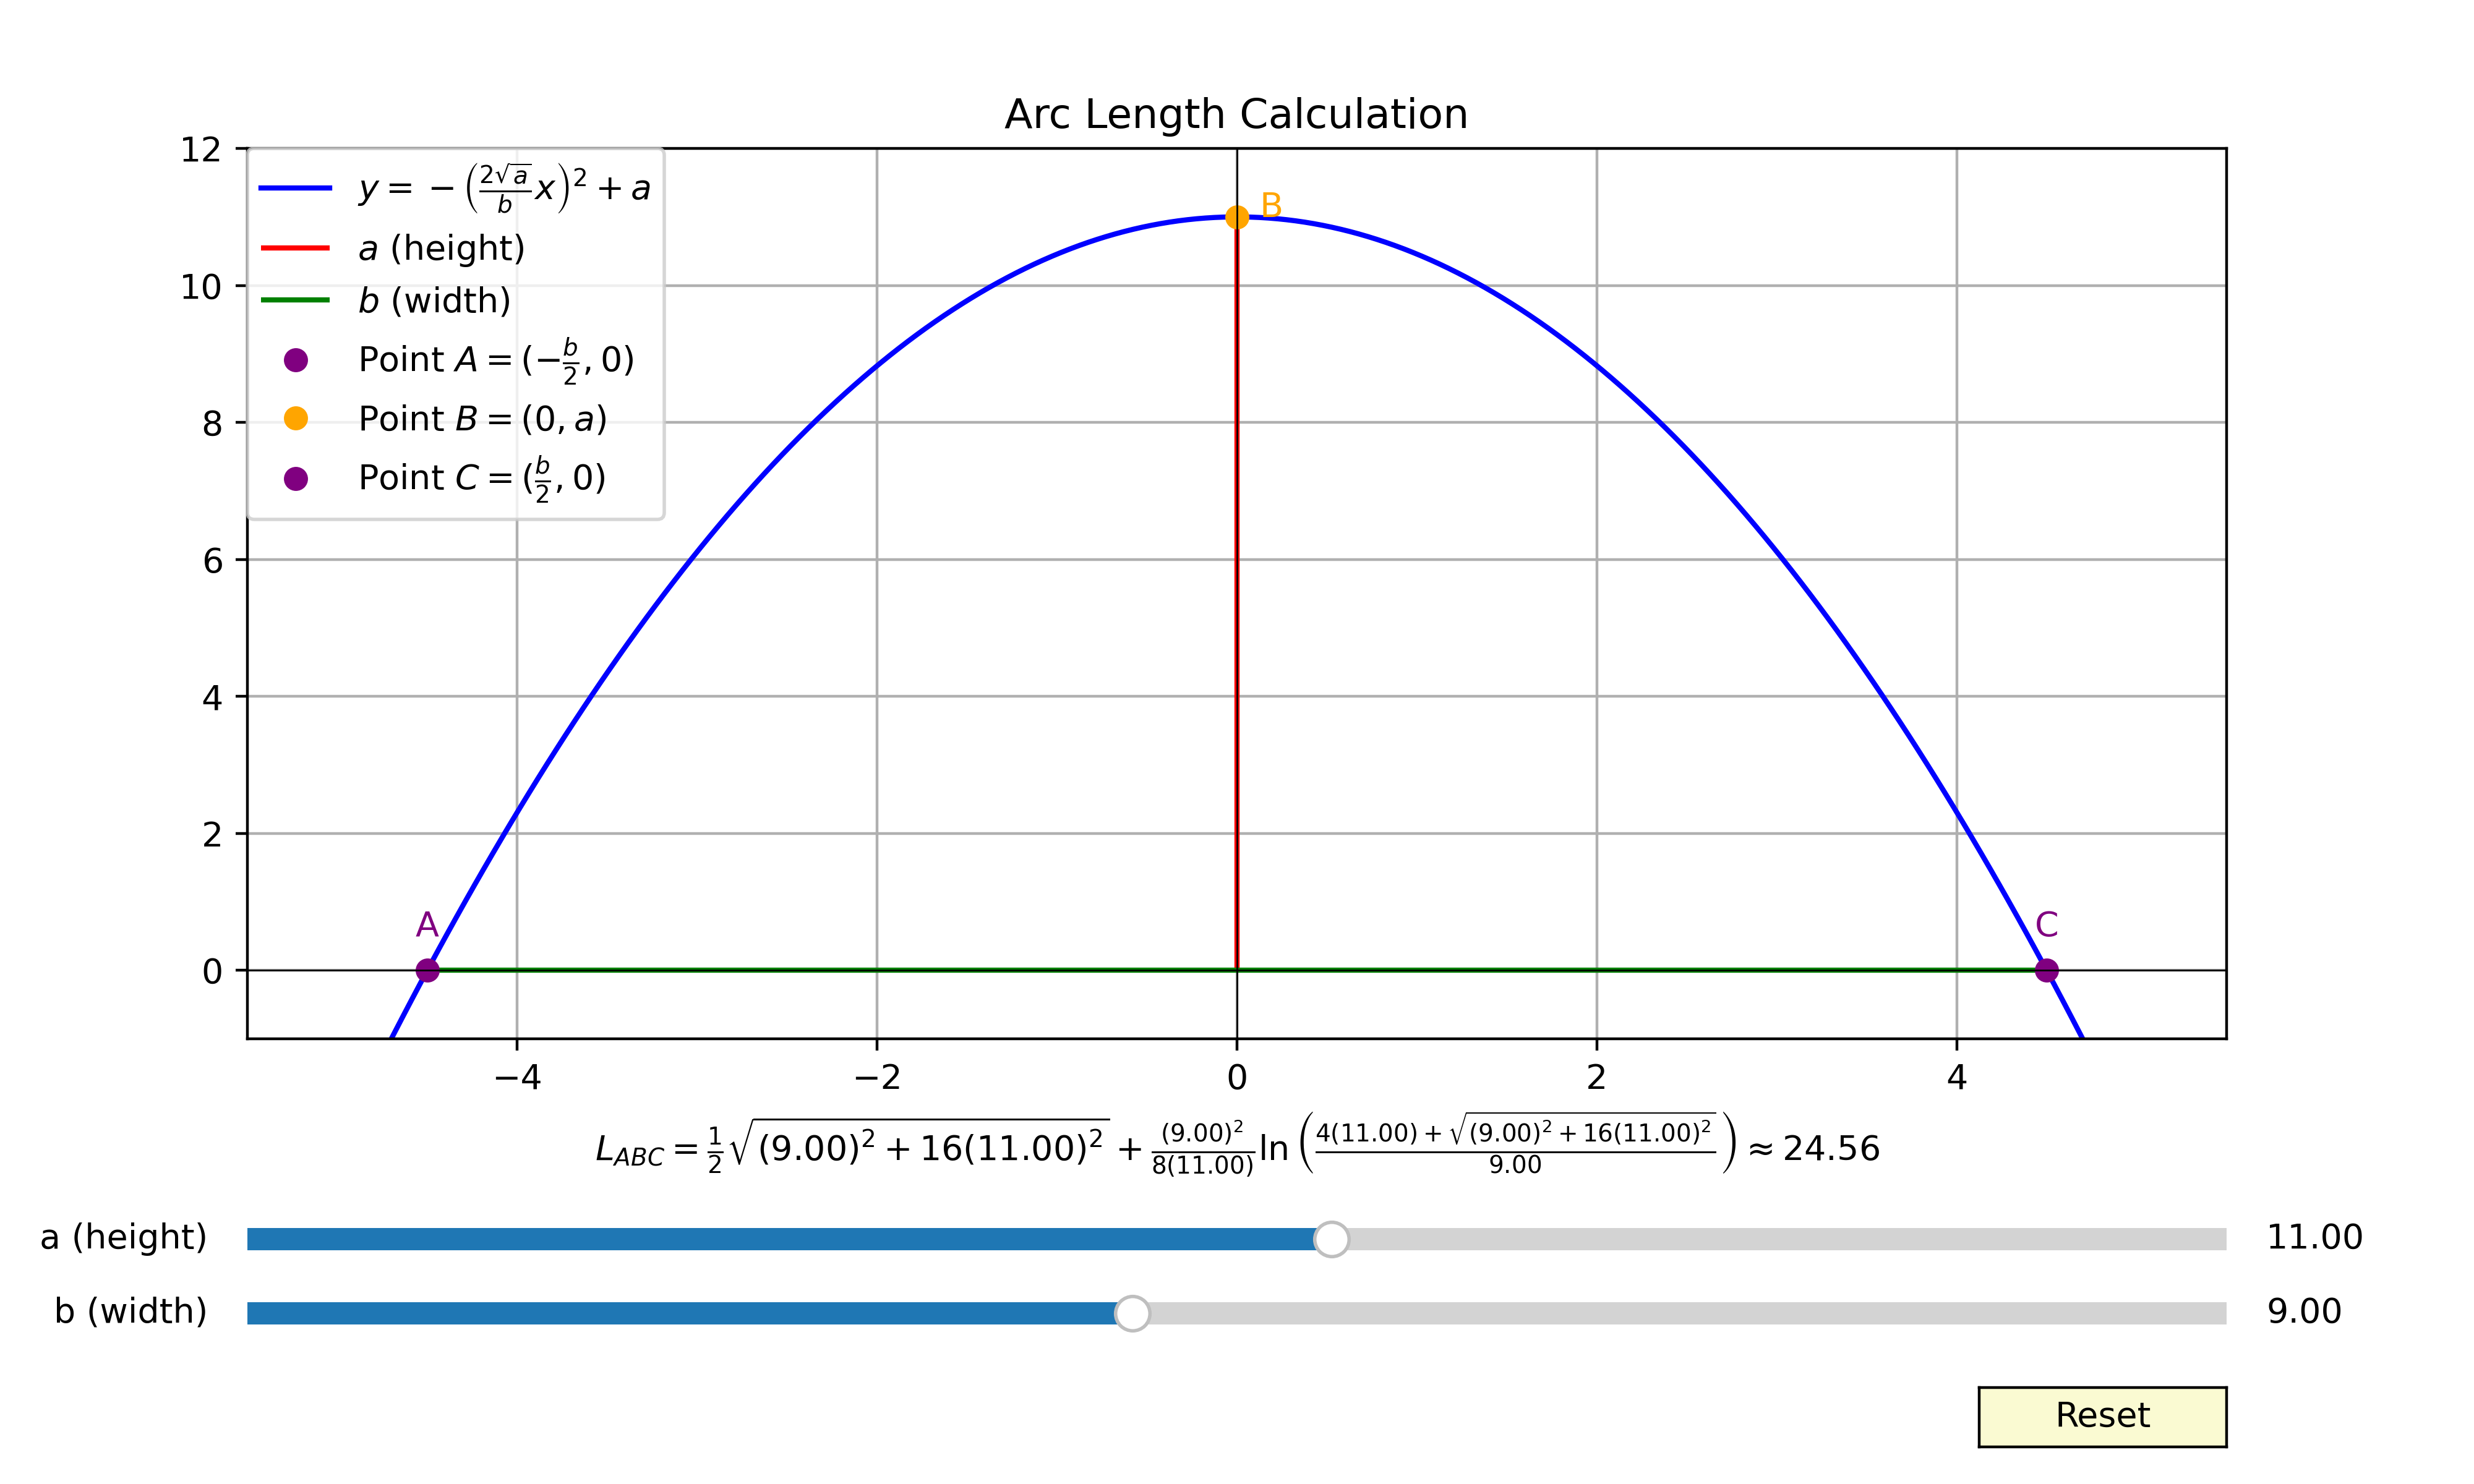
\includegraphics[scale=0.7]{figures/Figure_1.png}
    
    Since the goal was to utilize Matlab, I opted for this approach.\\[10pt] 
    However, this reduced Python version should suffice if a widely used and intuitive code is required.
    
    \lstinputlisting[style=mypythonstyle, title=\textbf{\textcolor{blue}{\texttt{\href{https://github.com/sakx7/mathcompuni/blob/main/scripts/q1_easy.py}{scripts/q1\_easy.py}}}}]{scripts/q1_easy.py}
            
    \newpage
   \begin{tcolorbox}[title=\color{black}{\section{Q1}}, colback=white, colframe=black!30!white, boxrule=0.4mm, width=1\textwidth]\centering
    The voltage difference \(V_{ab}\) between points \(a\) and \(b\) in the Wheatstone bridge circuit is given by the formula:
    
    \[
    V_{ab} = V \left(\frac{R_1 R_3 - R_2 R_4}{(R_1 + R_2)(R_3 + R_4)}\right)
    \]
    
    Write a universal, user-friendly program that calculates the voltage difference \(V_{ab}\). 
    
    Test your program using the following values:\\
    \vspace{1em}
    \hspace{8em}
    \centering
    \begin{minipage}{0.4\textwidth}
    \begin{itemize}[itemsep=-0.1cm]
        \item \(V = 14\) volts
        \item \(R_1 = 120.6\ \Omega\)
        \item \(R_2 = 119.3\ \Omega\)
        \item \(R_3 = 121.2\ \Omega\)
        \item \(R_4 = 118.8\ \Omega\)
    \end{itemize}
    \end{minipage}
    
    \end{tcolorbox}
    
\end{document}
